\section{Creating a dark state in a 3-level system\label{sec:dark_state}\cite{sillanpaa2009}\cite{abdumalikov2010}}
\iframe{We drive a 3-level system in such as way that one of it's states is never populated.}

We can use a flux qubit, solved in Chapter~\ref{sec:rfSquid}, for the 3-level system.
 
   \begin{figure}[h]
   	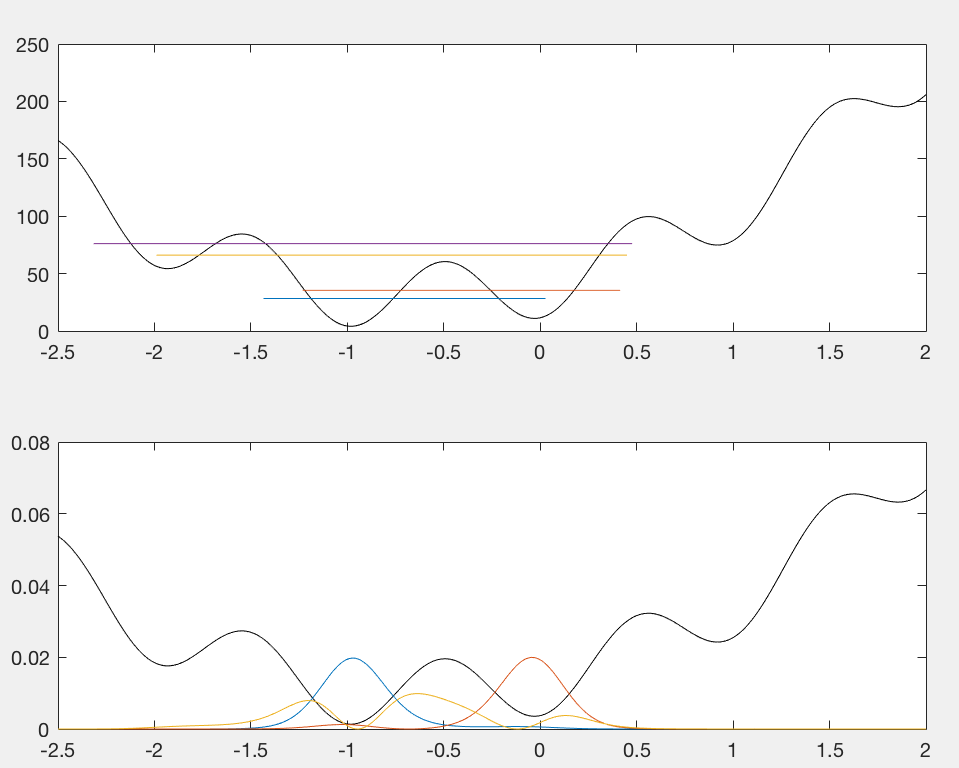
\includegraphics[height = 7cm]{rfSquid1} 	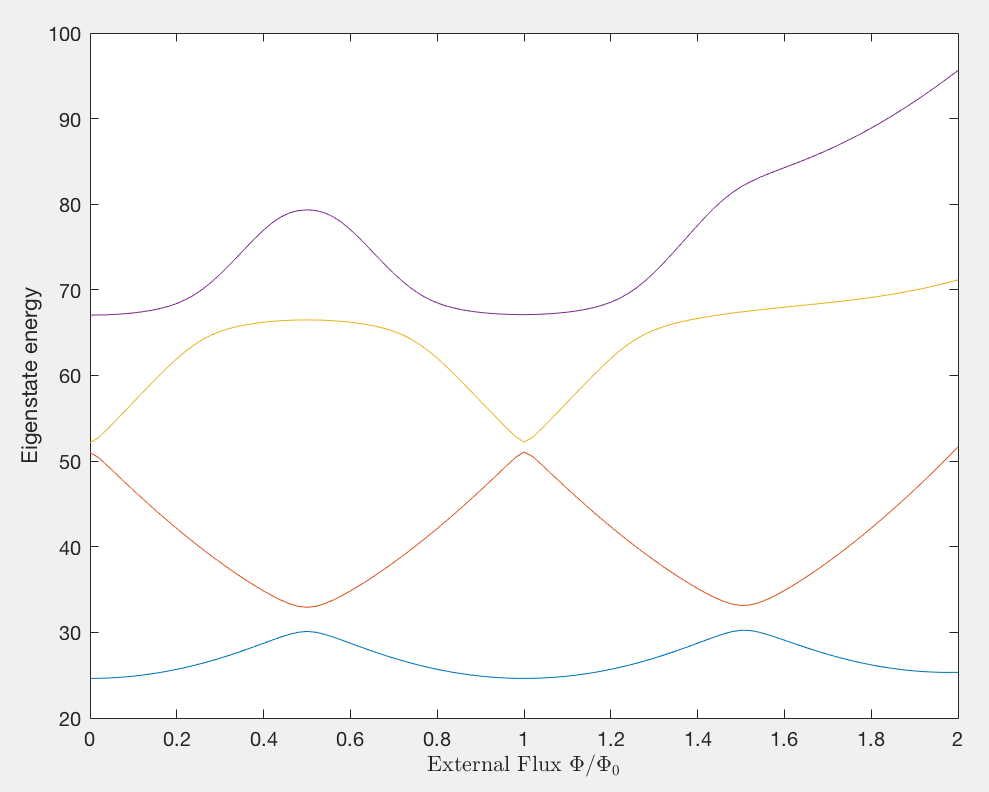
\includegraphics[height = 7cm]{rfSquid2}
   	\caption{\iket{0} migrates to the lower potential well as one increases the external flux. Black lines show the potential in the system.}
   	\label{fig:l3-myone}
   \end{figure}
  
 \subsection{Driving the three level atom\label{subsec:3LevelAtom}}  
  The Hamiltonian for a Three-Level atom, in a corresponding basis of eigenstates \iket{1}, \iket{2}, \iket{3}, by which the three levels are labelled, can be written as
  
  \begin{equation}
  \mathcal{H}_{\text{atom}} = \begin{pmatrix}
  E_1 & 0 & 0\\0& E_2 & 0 \\0&0&E_3
  \end{pmatrix}=\begin{pmatrix}
  E_3-\hbar\omega_{31} & 0 & 0\\0& E_3-\hbar\omega_{32} & 0 \\0&0&E_3
  \end{pmatrix},
  \label{rwaAtomicHamil}
  \end{equation}
  
  \noindent where $ \hbar\omega_{31} = E_3-E_1 $ and $ \hbar\omega_{32} = E_3-E_2$. Considering driving fields $ \Omega_{32} $, $ \Omega_{31} $ driving transitions \iket{2}\lra\iket{3} and \iket{1}\lra\iket{3} that arise due to capacitive or inductive coupling ($ \hbar\Omega_{ij} \propto \vartheta_{ij} $ is dervied in Chapter~\ref{sec:dipole_coupling})
  
  \begin{equation}
  \mathcal{H}_{\text{int}} = -\hbar\Omega_{31}\cos(\omega_{31}^{d}t) \begin{pmatrix}
  0 & 0 & 1\\0&0&0\\1&0&0
  \end{pmatrix}-\hbar\Omega_{32}\cos(\omega_{32}^{d}t) \begin{pmatrix}
  0 & 0 & 0\\0&0&1\\0&1&0
  \end{pmatrix},
  \label{rwaDriveHamiltonian}
  \end{equation}
  
  \noindent where the non-zero matrix elements indicate the states coupled by the fields. The total Hamiltonian, $ \mathcal{H}_{a} = \mathcal{H}_{\text{atom}}+\mathcal{H}_{\text{int}}$, is a sum of Eq.~\eqref{rwaAtomicHamil}, \eqref{rwaDriveHamiltonian}, written for convenience with complex exponentials,
  
  {\small \begin{equation}
  	\begin{aligned}
  	\mathcal{H}_{a}\ & {= \begin{pmatrix}
  		E_3-\hbar(\omega_{31}^{d}-\delta\omega_{31}) & 0 & -\frac{\hbar\Omega_{31}}{2}\bigg(e^{i\omega^{\text{d}}_{31}t}+e^{-i\omega^{\text{d}}_{31}t}\bigg)  \\   	0 & E_3-\hbar(\omega_{32}^{d}-\delta\omega_{32})  & -\frac{\hbar\Omega_{32}}{2}\bigg(e^{i\omega^{\text{d}}_{32}t}+e^{-i\omega^{\text{d}}_{32}t}\bigg)  \\   	-\frac{\hbar\Omega_{31}}{2}\bigg(e^{i\omega^{\text{d}}_{31}t}+e^{-i\omega^{\text{d}}_{31}t}\bigg)  & -\frac{\hbar\Omega_{32}}{2}\bigg(e^{i\omega^{\text{d}}_{32}t}+e^{-i\omega^{\text{d}}_{32}t}\bigg) & E_3 \\
  		\end{pmatrix}}\\& \qquad\qquad\qquad\qquad\qquad\qquad = \begin{pmatrix}
  	H_{11} & H_{12} & H_{13} \\   	H_{21} & H_{22} & H_{23} \\   	H_{31} & H_{32} & H_{33} \\
  	\end{pmatrix},
  	\end{aligned}
  	\label{rwaTotalHamiltonian}
  	\end{equation}}
  
  \noindent where $  \delta\omega_{31} = \omega_{31} - \omega^{\text{d}}_{31}, \delta\omega_{32} = \omega_{32} - \omega^{\text{d}}_{32}$ represent the detunings of the driving fields from the resonant frequencies of the atom. The Hamiltonian Eq.~\eqref{rwaTotalHamiltonian} governs the time evolution of the system state 
  
  \begin{equation}
  \ket{\varPsi} = c_1\ket{1}+c_2\ket{2}+c_3\ket{3},
  \end{equation} 
  
  \noindent through the standard \schrodinger equation, which takes on the matrix form
  
  \begin{equation}
  \begin{pmatrix}
  H_{11} & H_{12} & H_{13} \\   	H_{21} & H_{22} & H_{23} \\   	H_{31} & H_{32} & H_{33} \\
  \end{pmatrix}\begin{pmatrix}
  c_1\\c_2\\c_3
  \end{pmatrix} = i\hbar\begin{pmatrix}
  \dot{c_1} \\ \dot{c_2}\\\dot{c_3}
  \end{pmatrix}.
  \label{rwaTotalHamilMatrix}
  \end{equation}
  
  \noindent By applying a time dependent \red{\textbf{unitary transformation}}
  
  \begin{equation}
  \label{eqn:InteractionTransformation}
  \widetilde{c_i} = e^{i\phi_{i}(t)}c_i,
  \end{equation}
  
  \noindent where $ i=1,2,3 $, one can rewrite Eq.~\eqref{rwaTotalHamilMatrix} as
  
  \begin{equation}
  \begin{pmatrix}
  H_{11}-\hbar\dot{\phi}_1 & H_{12}e^{i\phi_{12}} & H_{13}e^{i\phi_{13}} \\  H_{21}e^{i\phi{21}} & H_{22}-\hbar\dot{\phi}_2 & H_{23}e^{i\phi{23}} \\   	H_{31}e^{i\phi{31}} & H_{32}e^{i\phi{32}} & H_{33}-\hbar\dot{\phi}_3 \\
  \end{pmatrix}\begin{pmatrix}
  \widetilde{c_1}\\\widetilde{c_2}\\\widetilde{c_3}
  \end{pmatrix} = i\hbar\begin{pmatrix}
  \dot{\widetilde{c_1}} \\ \dot{\widetilde{c_2}}\\\dot{\widetilde{c_3}}
  \end{pmatrix},
  \label{rawMatrixAfterTransformation}
  \end{equation}
  
  \noindent where $ e^{i\phi_{kj}} = e^{i(\phi_k-\phi_j)} $. Setting 
  
  \begin{equation}
  \phi_1 = \bigg(\frac{E_3}{\hbar}- \omega_{31}^d\bigg)t;\ \phi_2=\bigg(\frac{E_3}{\hbar}- \omega_{32}^d\bigg)t;\ \phi_3 = \frac{E_3}{\hbar}t,
  \label{rwaTransfomration}
  \end{equation}
  
  \noindent which effectively rotates the state vector components at the natural atomic evolution and detuning frequencies, \footnote{The full unitary transformation applied:
  	
  	$\qquad\qquad\quad U(t) = \exp\big[\frac{it}{\hbar}\left[({E_1}- \hbar\delta\omega_{31})\ketbra{1}{1}+({E_2}- \hbar\delta\omega_{32}\ketbra{2}{2})+E_{3}\ketbra{3}{3}\right]\big] $} will give a simple expression for the Hamiltonian
  
  \begin{equation}
  \widetilde{\mathcal{H}}_{a} = \begin{pmatrix}
  \hbar\delta\omega_{31} & 0 & -\frac{\hbar\Omega_{31}}{2}\\  0 & \hbar\delta\omega_{32} & -\frac{\hbar\Omega_{32}}{2} \\   	-\frac{\hbar\Omega_{31}}{2} & -\frac{\hbar\Omega_{32}}{2} & 0 \\
  \end{pmatrix} + \red{\begin{pmatrix}
  0 & 0 & -\frac{\hbar\Omega_{31}}{2}e^{-i2\omega^{d}_{31}t}\\  0 & 0 & -\frac{\hbar\Omega_{32}}{2}e^{-i2\omega^{d}_{32}t}  \\   	-\frac{\hbar\Omega_{31}}{2}e^{-i2\omega^{d}_{31}t} & -\frac{\hbar\Omega_{32}}{2}e^{-i2\omega^{d}_{32}t} & 0 \\
  \end{pmatrix}}.
  \label{rawTransformedFinal}
  \end{equation}
  
  \noindent In the rotating-wave-approximation, one ignores the contribution from the \red{fast rotating $ 2\omega^{d}_{31} $, $ 2\omega^{d}_{32} $} in the second term, since their oscillations will be averaged out at the time-scales of significant processes - physically they correspond to energy non-conserving processes. One is left with the following driving cases
  
  \begin{equation}
  \begin{aligned}
	  \label{rwaHamitlonianApprox}
	  \iket{1}\lra\iket{3} \text{ and } \iket{2}\lra\iket{3} & \quad 
	  	\widetilde{\mathcal{H}}_{a} = -\frac{\hbar}{2}
	  	\begin{pmatrix}
	  		-2\delta\omega_{31} & 0 & \Omega_{31}\\  0 & -2\delta\omega_{32} & \Omega_{32} \\   	\Omega_{31} & \Omega_{32} & 0
	  	\end{pmatrix};\\
	  \iket{1}\lra\iket{3} \text{ and } \iket{1}\lra\iket{2} & \quad 
	  	\widetilde{\mathcal{H}}_{b} = -\frac{\hbar}{2}
	  	\begin{pmatrix}
	  		0 & \Omega_{21} & \Omega_{31}\\  \Omega_{21} & 2\delta\omega_{21} & 0 \\   	\Omega_{31} & 0 & 2\delta\omega_{31}
	  	\end{pmatrix};\\
	  	\iket{1}\lra\iket{2} \text{ and } \iket{2}\lra\iket{3} & \quad 
	  		\widetilde{\mathcal{H}}_{c} = -\frac{\hbar}{2}
	  		\begin{pmatrix}
	  		0 & \Omega_{21} & 0\\  \Omega_{21} & 2\delta\omega_{21} & \Omega_{32} \\   	
	  		0 & \Omega_{32} & 2\delta\omega_{21} + 2\delta\omega_{32}
	  	\end{pmatrix}.
  \end{aligned}
  \end{equation}
  
  \noindent For various $ \delta\omega_{ij} \approxeq 0$, certain energy levels in the rotated frame become degenerate, shown in Fig.~\ref{theoRotation}b for a two level system. The off-diagonal terms induce a splitting $ \hbar\Omega $ between the eigenstates of the system,\footnote{For a Two-Level \iket{0}, \iket{1}, system,
  	
  	$\qquad\quad \mathcal{H} = \hbar\big(\begin{smallmatrix}0 & -\Omega/2\\-\Omega/2&0\end{smallmatrix}\big) $ has eigenenergies $ \pm\hbar\Omega $ and eigenstates $ \big(\iket{0}\mp\iket{1}\big)/\sqrt{2} $.} lifting this degeneracy. In the original unrotated frame, these Rabi splittings persist, resulting in a richer energy level structure as in Fig.~\ref{theoRotation}.
  
  \begin{figure}
  	\ifigure{4cm}{rotwave}
  	\caption{\textbf{The Rabi splitting of the energies in a Two-Level system.} A driving field with angular frequency $ \omega_{ij}^{d} $ and Rabi amplitude $ \Omega_{ij} $ in resonance with the atomic transition~$ \omega_{ij} $, couples the states \iket{i} and \iket{j}. In the rotated frame, the eigenstates $ \big(\iket{i}~\pm~\iket{j}\big)/\sqrt{2} $ are separated by an energy $ \hbar\Omega_{ij} $. Retuning to the original frame will map the Rabi splitting onto the original levels.}
  	\label{theoRotation}
  \end{figure}
  
  \newpage
  \subsection{Driving to the dark state\label{subsec:DoubleDrive}} 
  If $ \delta\omega_{32} = \delta\omega_{21} = 0 $ then Eq.~\eqref{rwaHamitlonianApprox} will read 
  
  \begin{equation}
	  \widetilde{\mathcal{H}}_{c} = -\frac{\hbar}{2}
	  \begin{pmatrix}
	  0 & \Omega_{21} & 0\\  \Omega_{21} & 0 & \Omega_{32} \\   	
	  0 & \Omega_{32} & 0
	  \end{pmatrix},
  \end{equation}
  
  \noindent with eigenvalues found from $ \det(\widetilde{\mathcal{H}}-\lambda\mathbb{I}) \equiv 0 $ and eigenvectors from $ (\widetilde{\mathcal{H}}-\lambda\mathbb{I})\vec{v} = 0 $:
   
   %  \eject \pdfpagewidth = 13in \pdfpageheight=10in
  \begin{equation}
	  \begin{aligned}
		  \red{E_0} &\red{= 0} & E_1 &= -\frac{\hbar}{2}\sqrt{\Omega_{21}^2+\Omega_{32}^2} & E_2 &= \frac{\hbar}{2}\sqrt{\Omega_{21}^2+\Omega_{32}^2}\\
		  \red{\vec{v}_0} & \red{= \frac{1}{\sqrt{\Omega_{21}^2 + \Omega_{32}^2}}
		  	\begin{pmatrix}
		  		\Omega_{32}\\0\\-\Omega_{21}
		  	\end{pmatrix}} & 
		  \vec{v}_1  & =
		  	\begin{pmatrix}
		  		\Omega_{21}\\ -\sqrt{\Omega_{21}^2 + \Omega_{32}^2} \\ \Omega_{32}
		  	\end{pmatrix} &
		 \vec{v}_2  & =
			 \begin{pmatrix}
		 		\Omega_{21}\\ \sqrt{\Omega_{21}^2 + \Omega_{32}^2} \\ \Omega_{32}
		 	\end{pmatrix},\\
	  \end{aligned}
  \end{equation}
   %    \eject \pdfpagewidth = 10in \pdfpageheight=10in
   
   \iframe{\noindent The state indicated in \red{red} is known as the dark state i.e. completely unpopulated \iket{1}. It happens when both the probe (\iket{0}\lra\iket{1}) and control (\iket{1}\lra\iket{2}) are on resonance:
   
   \[
   	\iket{\Psi_0} = \cos(\Theta)\iket{0} - \sin(\Theta)\iket{2};\qquad \tan(\Theta) = \frac{\Omega_{21}}{\Omega_{32}}.
   \]

	To get the ground state we do $ \sin(\Theta) = 0 \ra \Omega_p << \Omega_c $:
	\[
		\iket{\Psi_0}\approx \iket{0}
	\]
	}